% !TEX root = ../../main.tex

% --------------------------------------
% labels: \label{mil3:res:[type]:[name]}
% --------------------------------------
% PAST TENSE



% We present results for three wave numbers $k$, each of which representing its own regime: 
% \begin{itemize}
%     \item $k=0.001\unit{Mpc}$ represents the large scales
% \end{itemize}



The figures below demonstrate our results for three wave numbers $k$. 
% $k\in \{0.001,\,0.01,\, 0.1\} \unit{Mpc^{-1}}$

We present the absolute values of the matter perturbations in the upper panels of~\cref{mil3:res:fig:matter_perturbations}. The lower panels of said figure show the density and velocity perturbations for the photons.
\onecolumn
\begin{figure}
    \begin{subfigure}{0.49\linewidth}
        \centering
        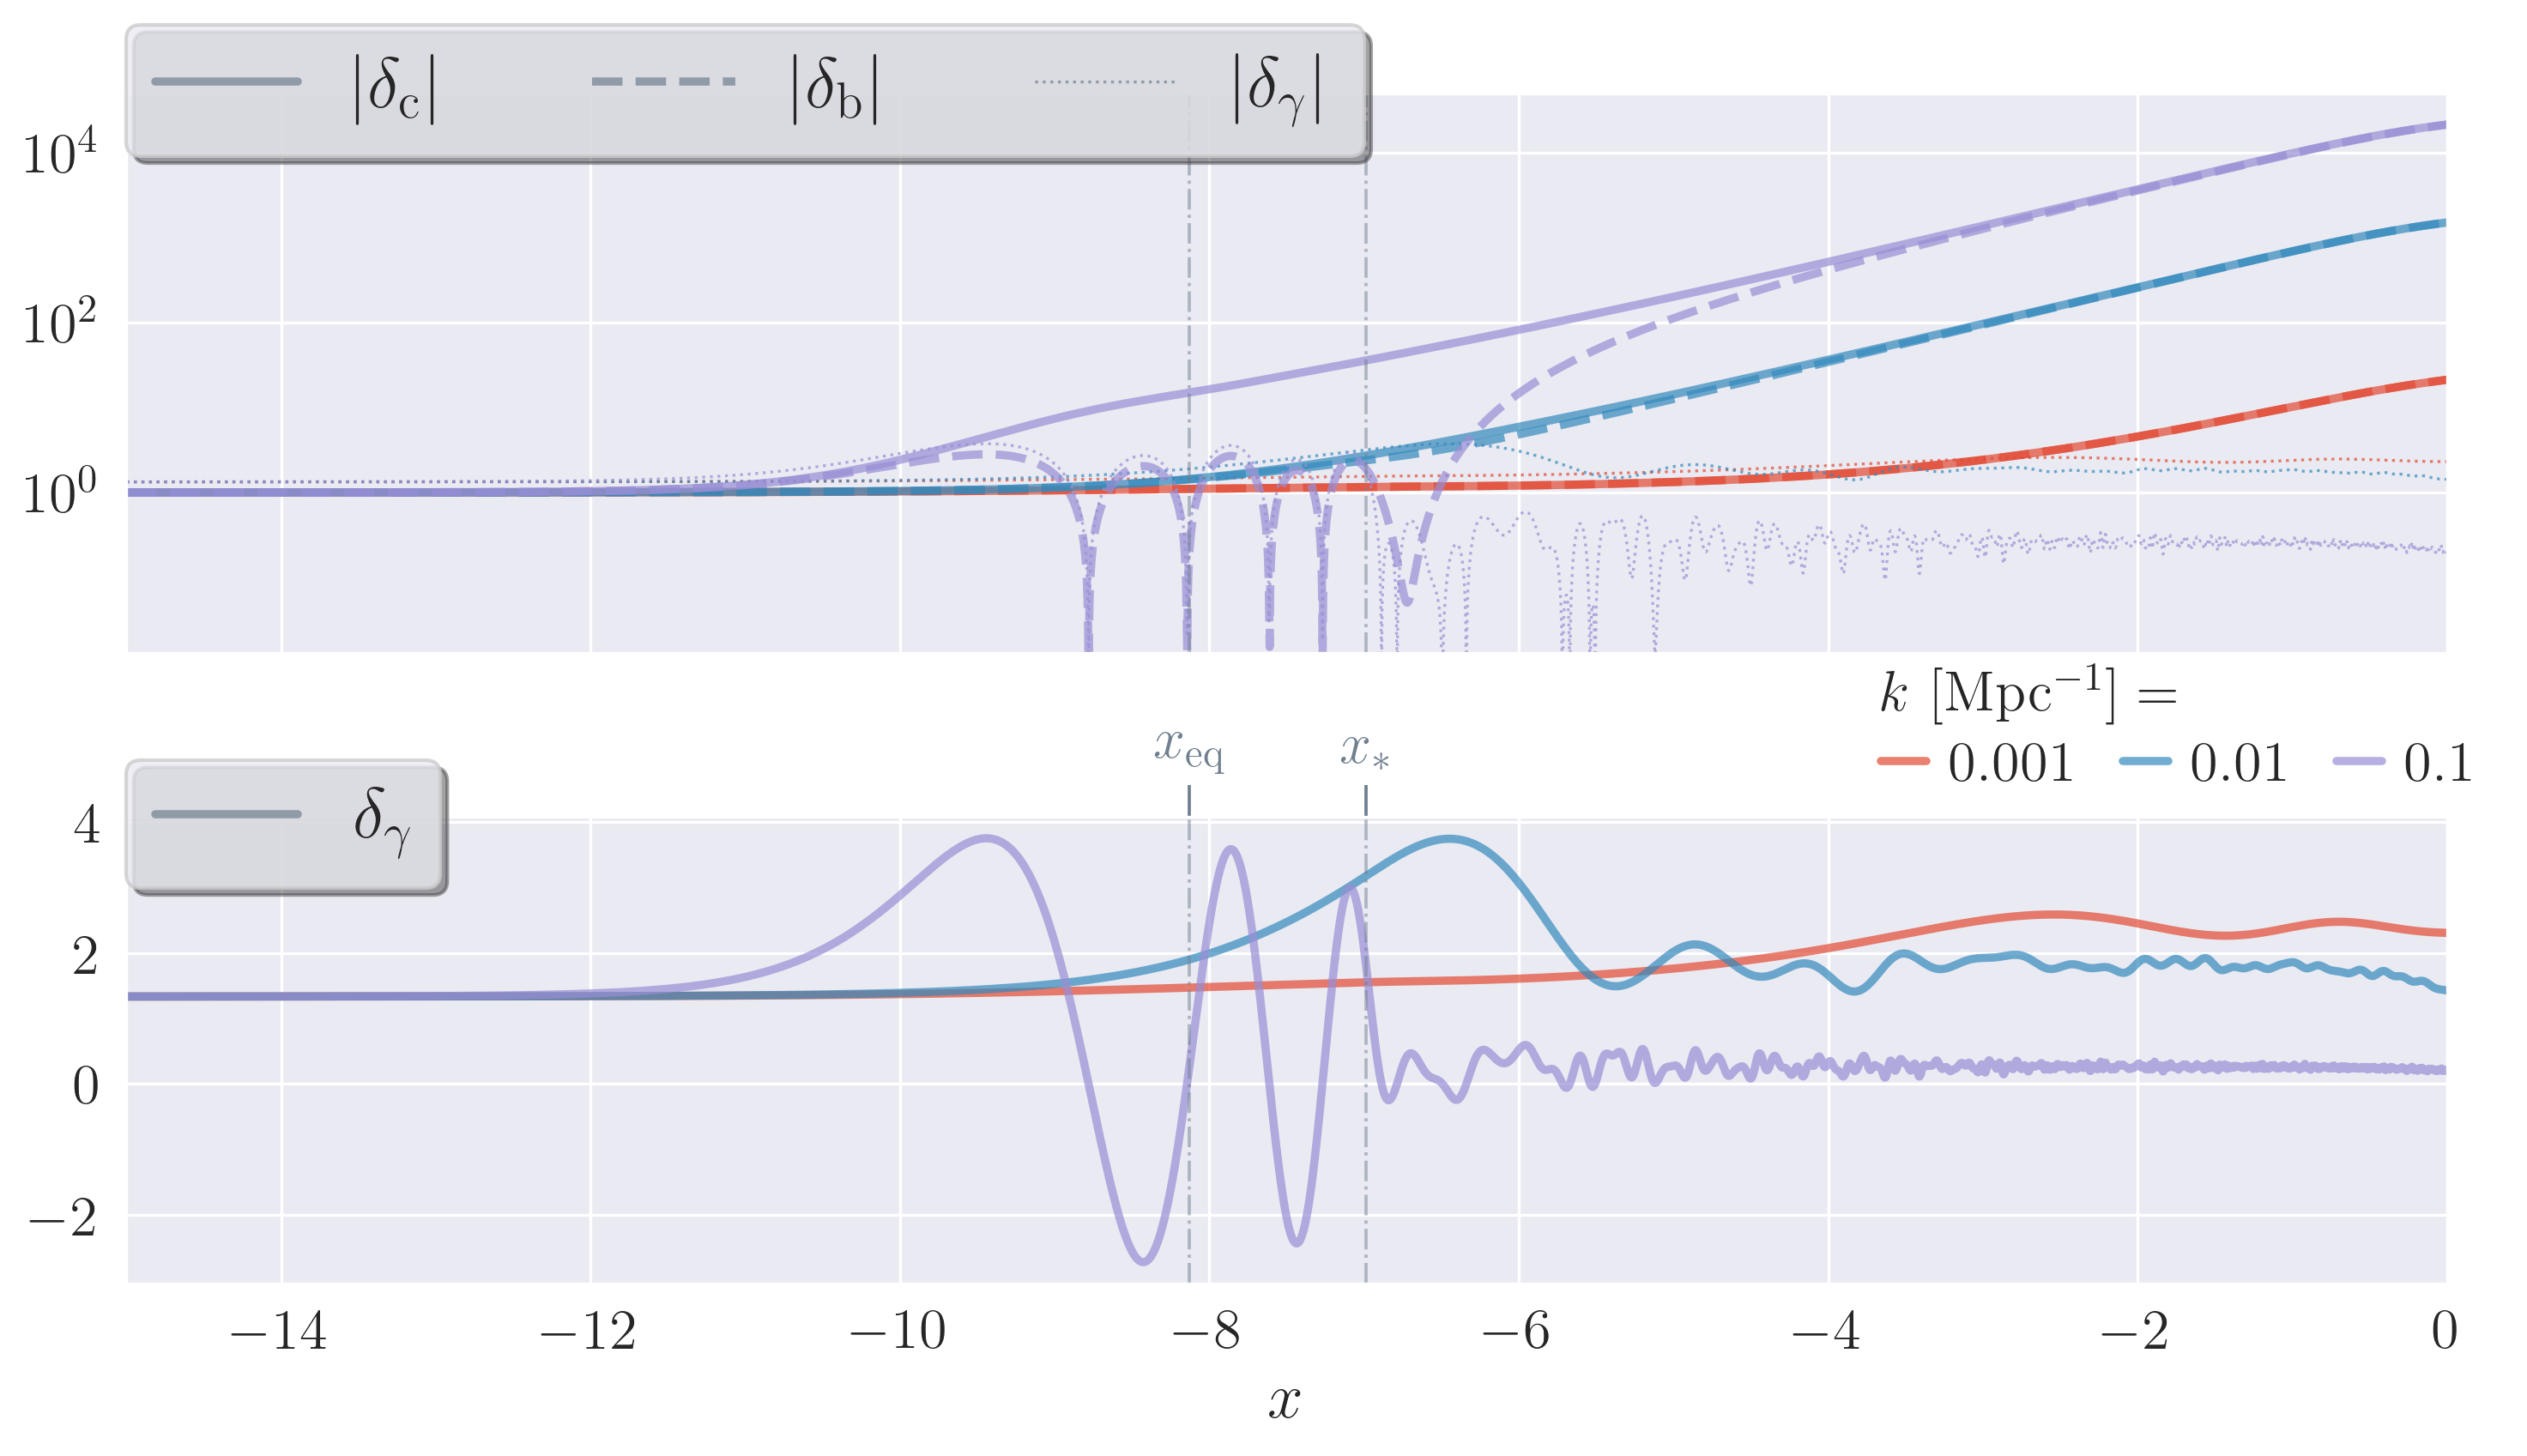
\includegraphics[width=\linewidth]{milestone3/density_perturbations.png} 
        \caption{\textcolor{orange}{CAPTION}}
    \label[fig]{mil3:res:fig:density_perturbations}
    \end{subfigure}
    \begin{subfigure}{0.49\linewidth}
        \centering
        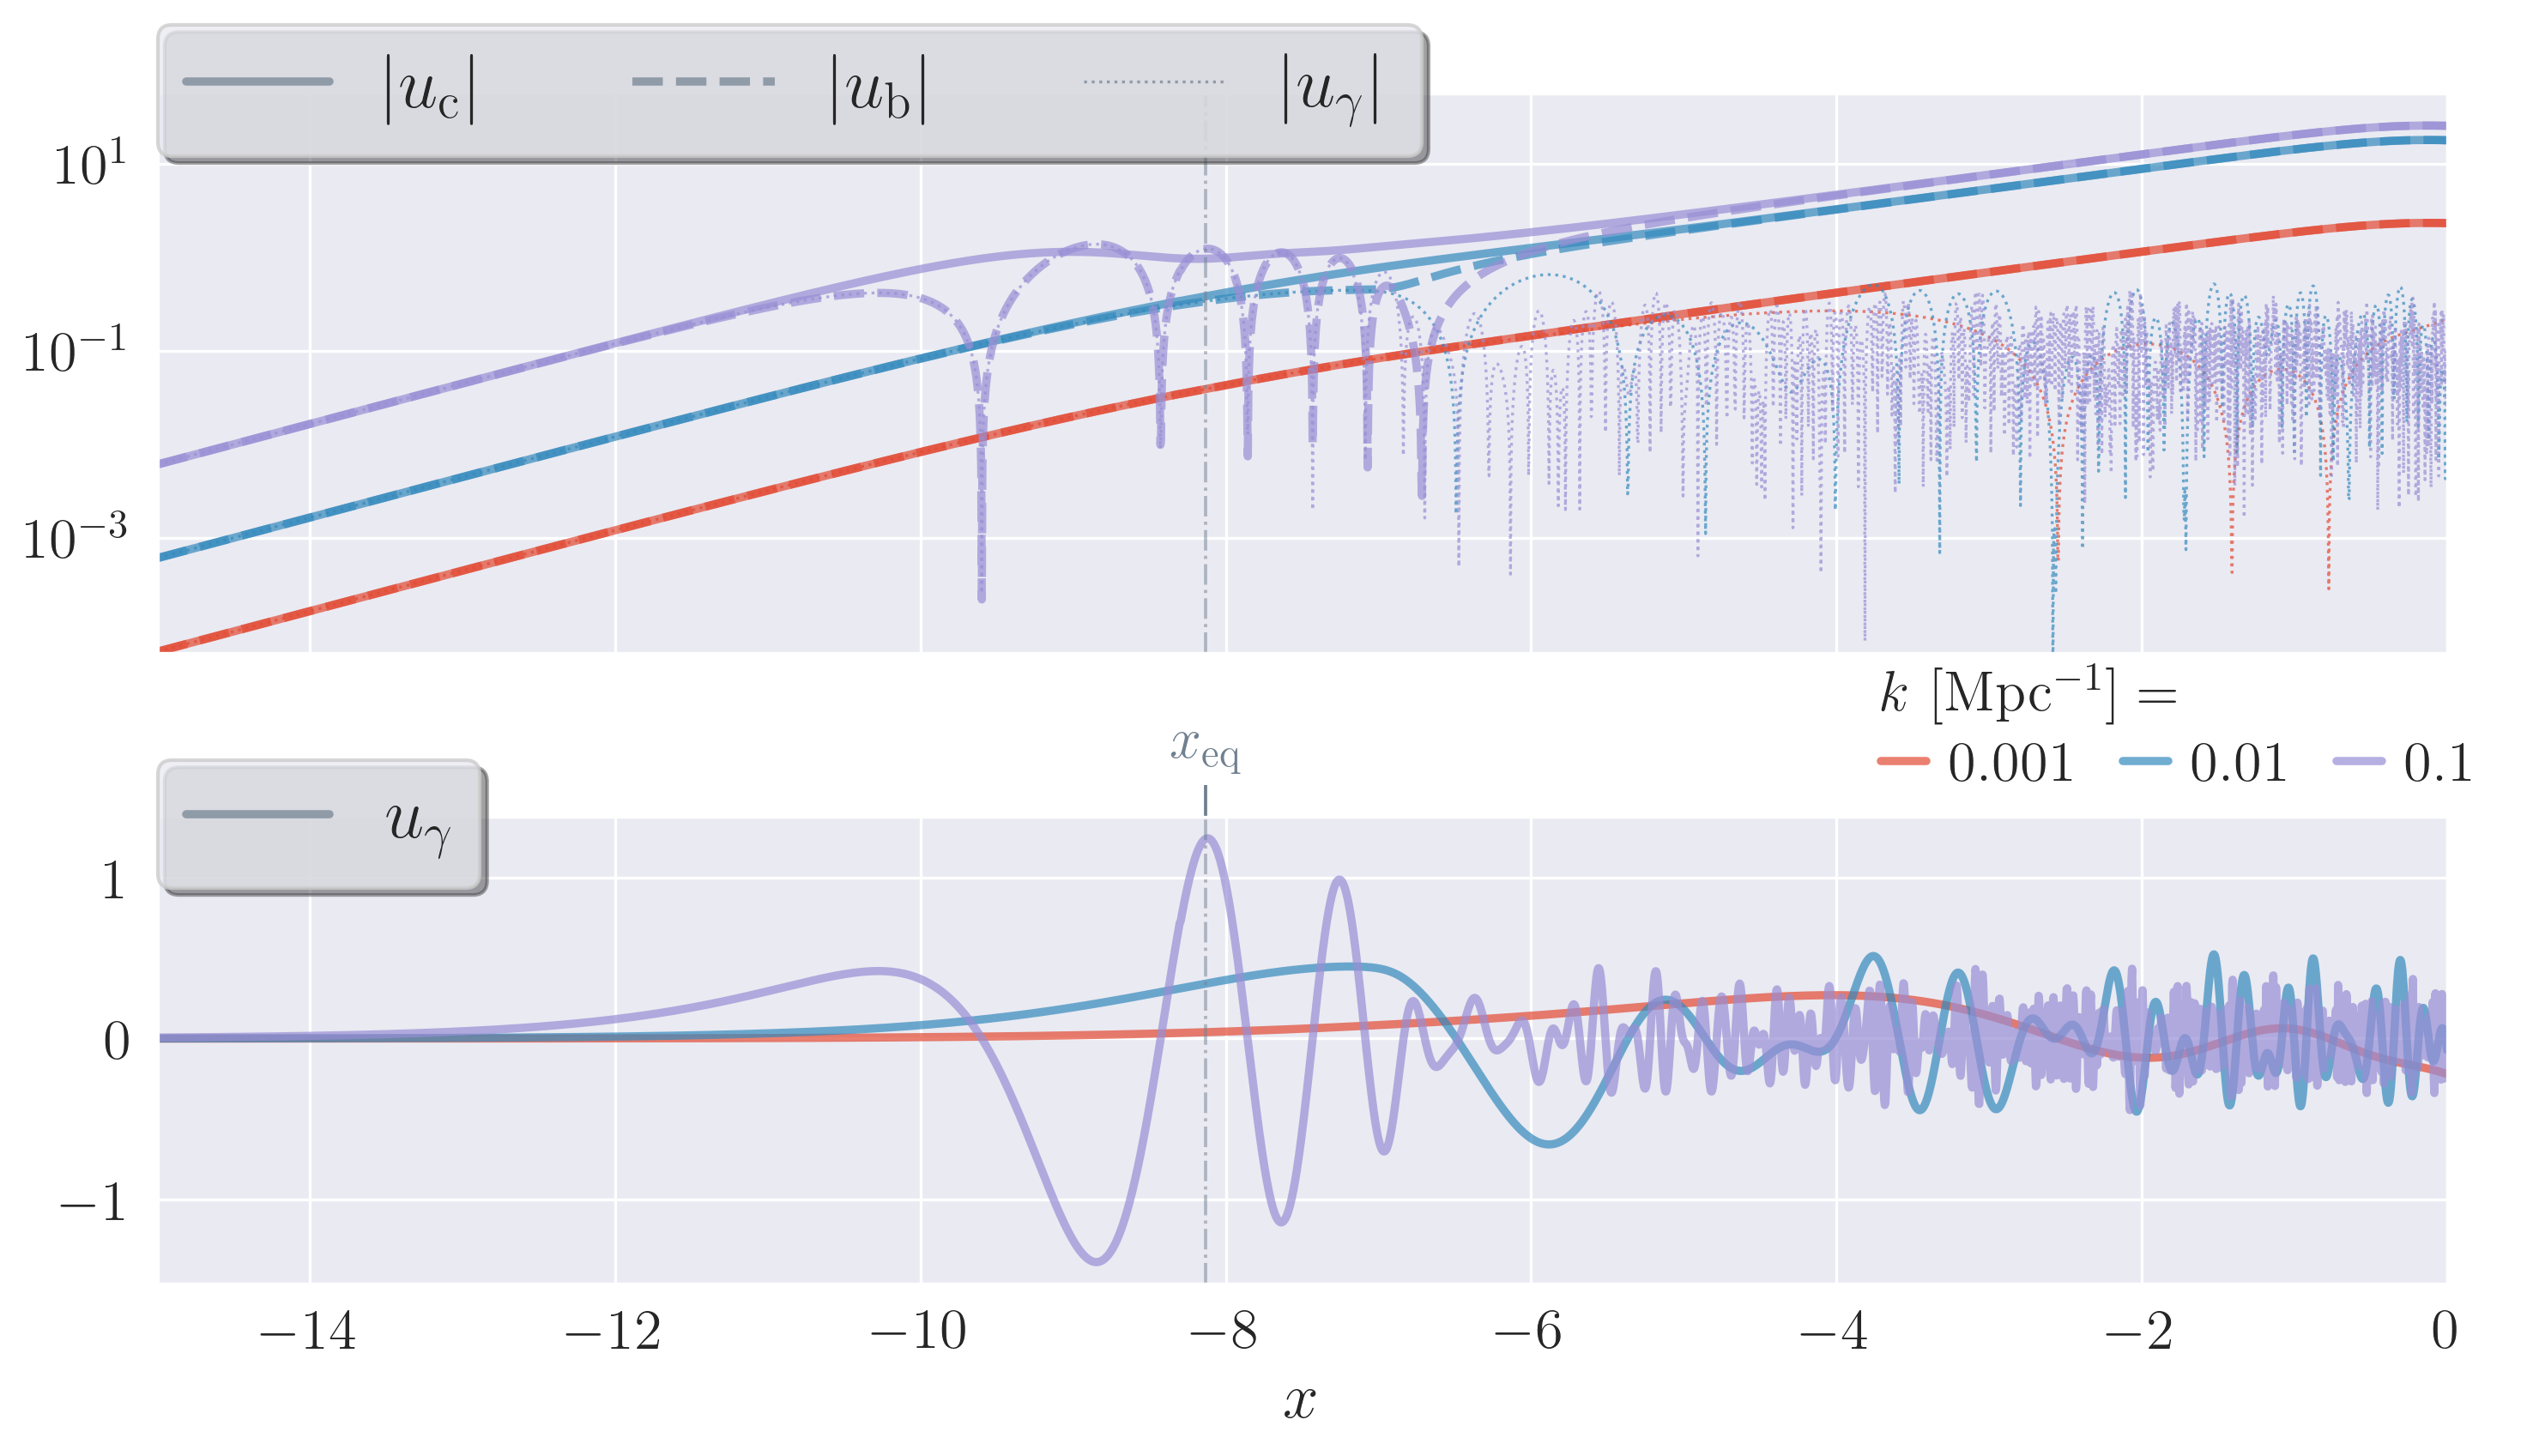
\includegraphics[width=\linewidth]{milestone3/velocity_perturbations.png} 
        \caption{\textcolor{orange}{CAPTION}} 
    \label[fig]{mil3:res:fig:velocity_perturbations}
    \end{subfigure}
    \caption{\textcolor{orange}{CAPTION (matter perturbations)}}
\label[fig]{mil3:res:fig:matter_perturbations}
\end{figure}
\twocolumn


The photon quadrupole is plotted in~\cref{mil3:res:fig:photon_quadrupole}.
\begin{figure}[!ht]
    \centering
    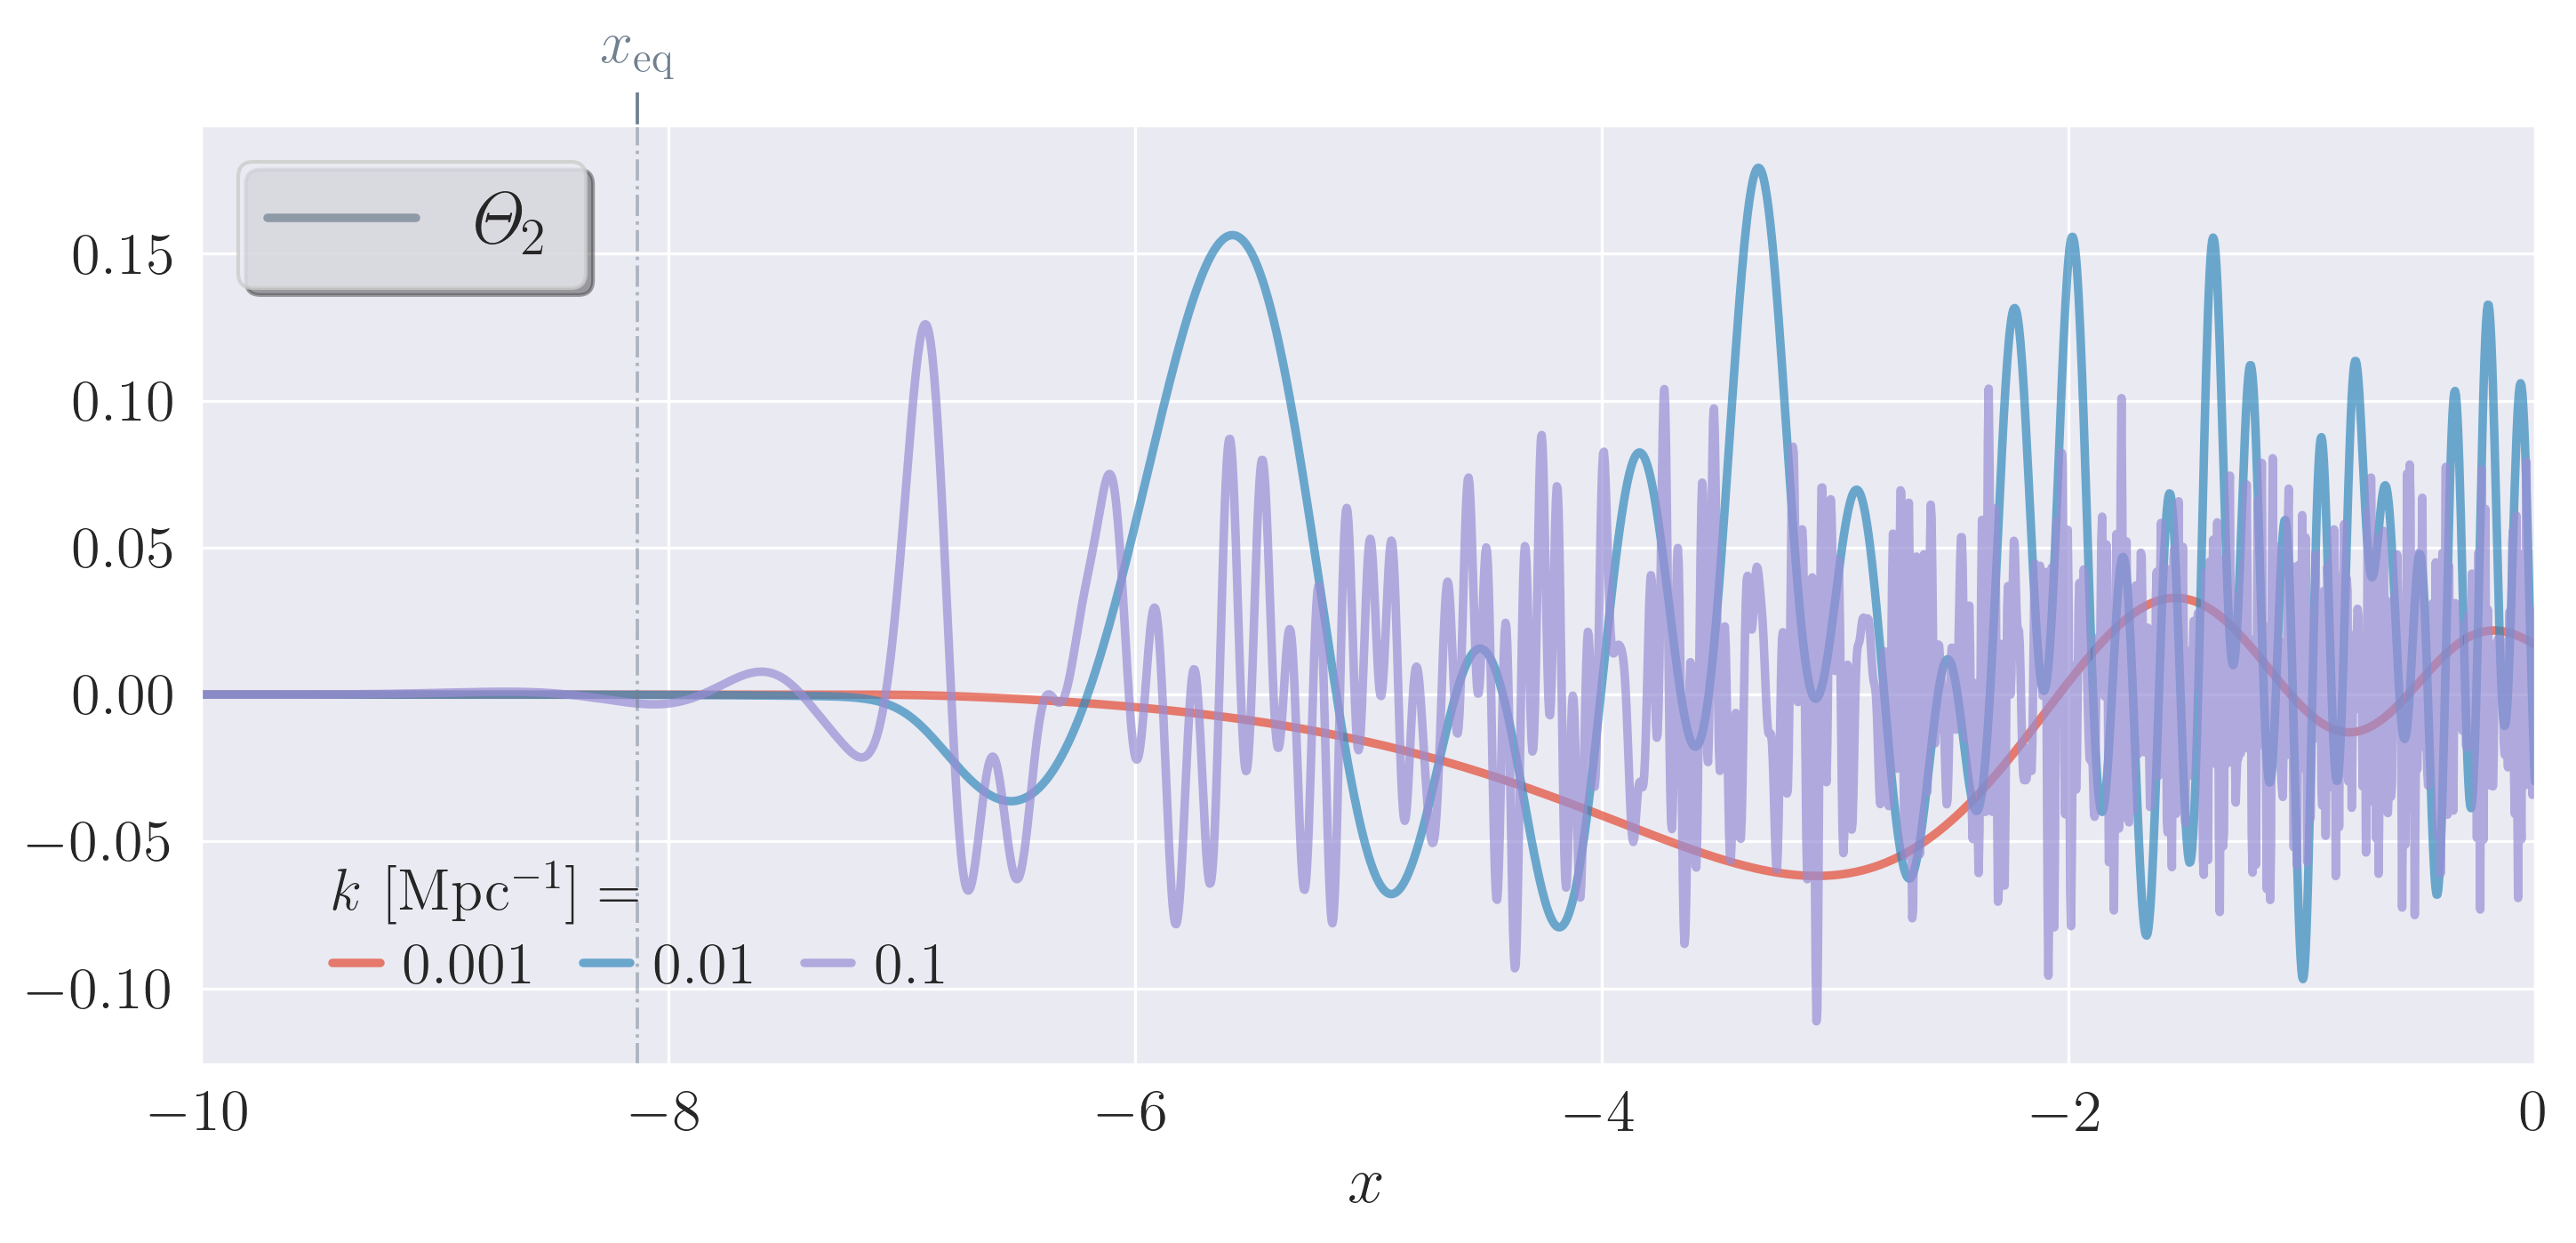
\includegraphics[width=\linewidth]{milestone3/photon_quadrupole.png} 
    \caption{\textcolor{orange}{CAPTION}} 
    \label[fig]{mil3:res:fig:photon_quadrupole}
\end{figure}

\cref{mil3:res:fig:gravitational_potential} shows the gravitational potential as well as the sum of this and \colorbox{blue}{\textcolor{orange}{XXX}} as functions of logarithmic expansion factor for our chosen wave numbers.
\begin{figure}[!ht]
    \centering
    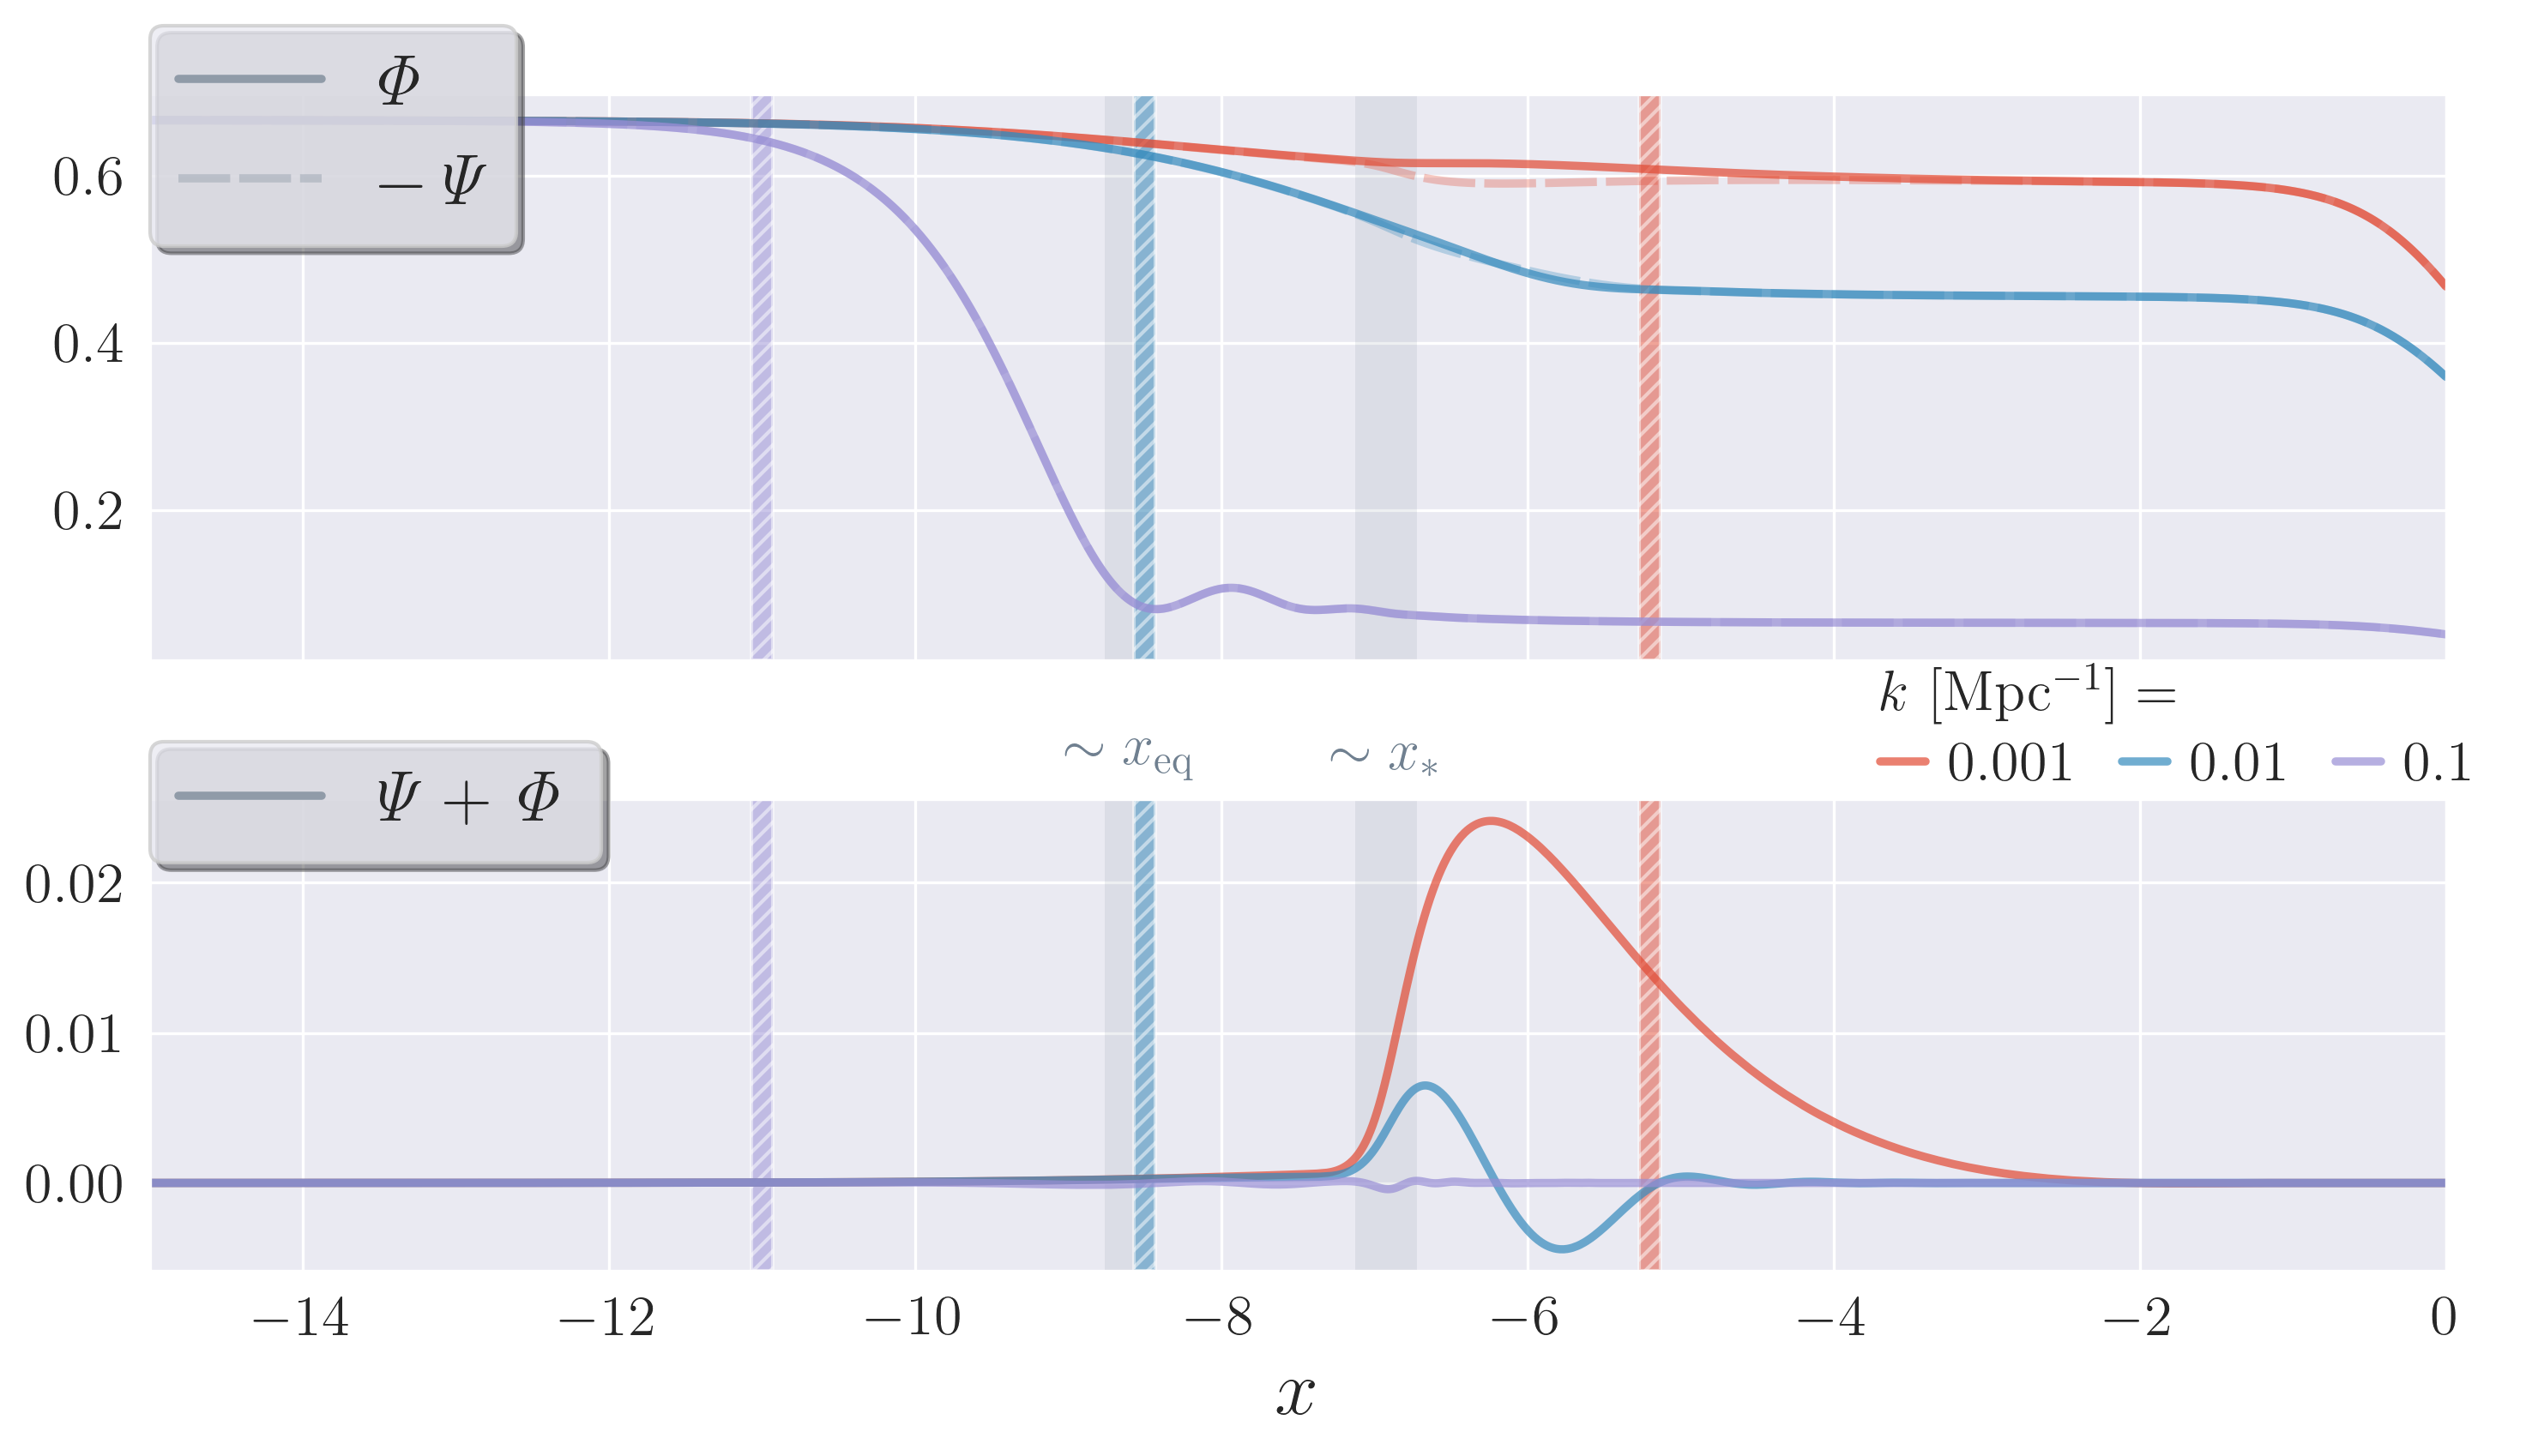
\includegraphics[width=\linewidth]{milestone3/gravitational_potential.png} 
    \caption{\textcolor{orange}{CAPTION}} 
    \label[fig]{mil3:res:fig:gravitational_potential}
\end{figure}
